    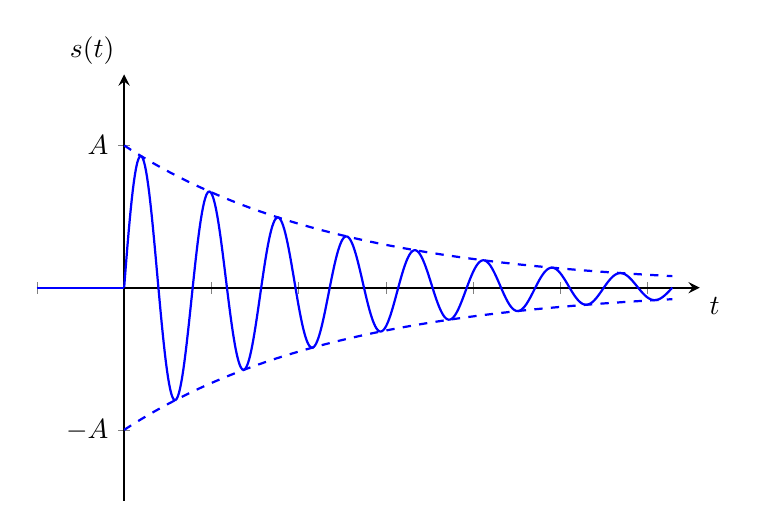
\begin{tikzpicture}
        \begin{axis}[
        axis line style = thick,
        clip=false,
        height=7cm,
        width=10cm,
        axis x line=center,
        axis y line=center,
        xmin=-2,
        xmax=4.2*pi,
        ymin=-1.5,
        ymax=1.5,
        xlabel={$t$},
        ylabel={$s(t)$},
        xlabel style={below right},
        ylabel style={above left},
        ytick={-1,1},
        yticklabels={$-A$,$A$},
        xtick={},
        xticklabels={},
        ]

            \addplot [thick,color=blue,domain=-2:0, samples=11,unbounded coords=jump]{0};
            \addplot [thick,color=blue,domain=0:4*pi, samples=501,unbounded coords=jump]{exp(-0.2*x)*sin(4*deg(x))};
            \addplot [dashed,thick,color=blue,domain=0:4*pi, samples=501,unbounded coords=jump]{exp(-0.2*x)};
            \addplot [dashed,thick,color=blue,domain=0:4*pi, samples=501,unbounded coords=jump]{-exp(-0.2*x)};
            %\addplot [thick,color=red,domain=0:4*pi, samples=501,unbounded coords=jump]{exp(-0.2*x)*sin(deg(4*x-pi*0.5))};
%            \draw[blue,] (axis cs:pi*0.5,1) -- (axis cs:pi*0.5,1.25);
%            \draw[blue] (axis cs:pi*2.5,1) -- (axis cs:pi*2.5,1.25);
%            \draw[blue,ultra thick, latex-latex] (axis cs:pi*0.5,1.2) --node[above,yshift=+0.2em]{$\dfrac{2\pi}{\omega}$} (axis cs:pi*2.5,1.2);
%            \draw[blue,] (axis cs:pi*1.5,-1) -- (axis cs:pi*1.5,-1.25);
%            \draw[blue] (axis cs:pi*1.5+pi*0.5,-1) -- (axis cs:pi*1.5+pi*0.5,-1.25);
%            \draw[blue,ultra thick, latex-latex] (axis cs:pi*1.5,-1.2) --node[below,yshift=-0.2em]{$\dfrac{\Delta\phi}{\omega}$} (axis cs:pi*1.5+pi*0.5,-1.2);
        \end{axis}
    \end{tikzpicture}
